


% Header, overrides base

    % Make sure that the sphinx doc style knows who it inherits from.
    \def\sphinxdocclass{article}

    % Declare the document class
    \documentclass[letterpaper,10pt,english]{/Users/ayocom/anaconda/lib/python2.7/site-packages/sphinx/texinputs/sphinxhowto}

    % Imports
    \usepackage[utf8]{inputenc}
    \DeclareUnicodeCharacter{00A0}{\\nobreakspace}
    \usepackage[T1]{fontenc}
    \usepackage{babel}
    \usepackage{times}
    \usepackage{import}
    \usepackage[Bjarne]{/Users/ayocom/anaconda/lib/python2.7/site-packages/sphinx/texinputs/fncychap}
    \usepackage{longtable}
    \usepackage{/Users/ayocom/anaconda/lib/python2.7/site-packages/sphinx/texinputs/sphinx}
    \usepackage{multirow}

    \usepackage{amsmath}
    \usepackage{amssymb}
    \usepackage{ucs}
    \usepackage{enumerate}

    % Used to make the Input/Output rules follow around the contents.
    \usepackage{needspace}

    % Pygments requirements
    \usepackage{fancyvrb}
    \usepackage{color}
    % ansi colors additions
    \definecolor{darkgreen}{rgb}{.12,.54,.11}
    \definecolor{lightgray}{gray}{.95}
    \definecolor{brown}{rgb}{0.54,0.27,0.07}
    \definecolor{purple}{rgb}{0.5,0.0,0.5}
    \definecolor{darkgray}{gray}{0.25}
    \definecolor{lightred}{rgb}{1.0,0.39,0.28}
    \definecolor{lightgreen}{rgb}{0.48,0.99,0.0}
    \definecolor{lightblue}{rgb}{0.53,0.81,0.92}
    \definecolor{lightpurple}{rgb}{0.87,0.63,0.87}
    \definecolor{lightcyan}{rgb}{0.5,1.0,0.83}

    % Needed to box output/input
    \usepackage{tikz}
        \usetikzlibrary{calc,arrows,shadows}
    \usepackage[framemethod=tikz]{mdframed}

    \usepackage{alltt}

    % Used to load and display graphics
    \usepackage{graphicx}
    \graphicspath{ {figs/} }
    \usepackage[Export]{adjustbox} % To resize

    % used so that images for notebooks which have spaces in the name can still be included
    \usepackage{grffile}


    % For formatting output while also word wrapping.
    \usepackage{listings}
    \lstset{breaklines=true}
    \lstset{basicstyle=\small\ttfamily}
    \def\smaller{\fontsize{9.5pt}{9.5pt}\selectfont}

    %Pygments definitions
    
\makeatletter
\def\PY@reset{\let\PY@it=\relax \let\PY@bf=\relax%
    \let\PY@ul=\relax \let\PY@tc=\relax%
    \let\PY@bc=\relax \let\PY@ff=\relax}
\def\PY@tok#1{\csname PY@tok@#1\endcsname}
\def\PY@toks#1+{\ifx\relax#1\empty\else%
    \PY@tok{#1}\expandafter\PY@toks\fi}
\def\PY@do#1{\PY@bc{\PY@tc{\PY@ul{%
    \PY@it{\PY@bf{\PY@ff{#1}}}}}}}
\def\PY#1#2{\PY@reset\PY@toks#1+\relax+\PY@do{#2}}

\expandafter\def\csname PY@tok@gd\endcsname{\def\PY@tc##1{\textcolor[rgb]{0.63,0.00,0.00}{##1}}}
\expandafter\def\csname PY@tok@gu\endcsname{\let\PY@bf=\textbf\def\PY@tc##1{\textcolor[rgb]{0.50,0.00,0.50}{##1}}}
\expandafter\def\csname PY@tok@gt\endcsname{\def\PY@tc##1{\textcolor[rgb]{0.00,0.27,0.87}{##1}}}
\expandafter\def\csname PY@tok@gs\endcsname{\let\PY@bf=\textbf}
\expandafter\def\csname PY@tok@gr\endcsname{\def\PY@tc##1{\textcolor[rgb]{1.00,0.00,0.00}{##1}}}
\expandafter\def\csname PY@tok@cm\endcsname{\let\PY@it=\textit\def\PY@tc##1{\textcolor[rgb]{0.25,0.50,0.50}{##1}}}
\expandafter\def\csname PY@tok@vg\endcsname{\def\PY@tc##1{\textcolor[rgb]{0.10,0.09,0.49}{##1}}}
\expandafter\def\csname PY@tok@m\endcsname{\def\PY@tc##1{\textcolor[rgb]{0.40,0.40,0.40}{##1}}}
\expandafter\def\csname PY@tok@mh\endcsname{\def\PY@tc##1{\textcolor[rgb]{0.40,0.40,0.40}{##1}}}
\expandafter\def\csname PY@tok@go\endcsname{\def\PY@tc##1{\textcolor[rgb]{0.53,0.53,0.53}{##1}}}
\expandafter\def\csname PY@tok@ge\endcsname{\let\PY@it=\textit}
\expandafter\def\csname PY@tok@vc\endcsname{\def\PY@tc##1{\textcolor[rgb]{0.10,0.09,0.49}{##1}}}
\expandafter\def\csname PY@tok@il\endcsname{\def\PY@tc##1{\textcolor[rgb]{0.40,0.40,0.40}{##1}}}
\expandafter\def\csname PY@tok@cs\endcsname{\let\PY@it=\textit\def\PY@tc##1{\textcolor[rgb]{0.25,0.50,0.50}{##1}}}
\expandafter\def\csname PY@tok@cp\endcsname{\def\PY@tc##1{\textcolor[rgb]{0.74,0.48,0.00}{##1}}}
\expandafter\def\csname PY@tok@gi\endcsname{\def\PY@tc##1{\textcolor[rgb]{0.00,0.63,0.00}{##1}}}
\expandafter\def\csname PY@tok@gh\endcsname{\let\PY@bf=\textbf\def\PY@tc##1{\textcolor[rgb]{0.00,0.00,0.50}{##1}}}
\expandafter\def\csname PY@tok@ni\endcsname{\let\PY@bf=\textbf\def\PY@tc##1{\textcolor[rgb]{0.60,0.60,0.60}{##1}}}
\expandafter\def\csname PY@tok@nl\endcsname{\def\PY@tc##1{\textcolor[rgb]{0.63,0.63,0.00}{##1}}}
\expandafter\def\csname PY@tok@nn\endcsname{\let\PY@bf=\textbf\def\PY@tc##1{\textcolor[rgb]{0.00,0.00,1.00}{##1}}}
\expandafter\def\csname PY@tok@no\endcsname{\def\PY@tc##1{\textcolor[rgb]{0.53,0.00,0.00}{##1}}}
\expandafter\def\csname PY@tok@na\endcsname{\def\PY@tc##1{\textcolor[rgb]{0.49,0.56,0.16}{##1}}}
\expandafter\def\csname PY@tok@nb\endcsname{\def\PY@tc##1{\textcolor[rgb]{0.00,0.50,0.00}{##1}}}
\expandafter\def\csname PY@tok@nc\endcsname{\let\PY@bf=\textbf\def\PY@tc##1{\textcolor[rgb]{0.00,0.00,1.00}{##1}}}
\expandafter\def\csname PY@tok@nd\endcsname{\def\PY@tc##1{\textcolor[rgb]{0.67,0.13,1.00}{##1}}}
\expandafter\def\csname PY@tok@ne\endcsname{\let\PY@bf=\textbf\def\PY@tc##1{\textcolor[rgb]{0.82,0.25,0.23}{##1}}}
\expandafter\def\csname PY@tok@nf\endcsname{\def\PY@tc##1{\textcolor[rgb]{0.00,0.00,1.00}{##1}}}
\expandafter\def\csname PY@tok@si\endcsname{\let\PY@bf=\textbf\def\PY@tc##1{\textcolor[rgb]{0.73,0.40,0.53}{##1}}}
\expandafter\def\csname PY@tok@s2\endcsname{\def\PY@tc##1{\textcolor[rgb]{0.73,0.13,0.13}{##1}}}
\expandafter\def\csname PY@tok@vi\endcsname{\def\PY@tc##1{\textcolor[rgb]{0.10,0.09,0.49}{##1}}}
\expandafter\def\csname PY@tok@nt\endcsname{\let\PY@bf=\textbf\def\PY@tc##1{\textcolor[rgb]{0.00,0.50,0.00}{##1}}}
\expandafter\def\csname PY@tok@nv\endcsname{\def\PY@tc##1{\textcolor[rgb]{0.10,0.09,0.49}{##1}}}
\expandafter\def\csname PY@tok@s1\endcsname{\def\PY@tc##1{\textcolor[rgb]{0.73,0.13,0.13}{##1}}}
\expandafter\def\csname PY@tok@sh\endcsname{\def\PY@tc##1{\textcolor[rgb]{0.73,0.13,0.13}{##1}}}
\expandafter\def\csname PY@tok@sc\endcsname{\def\PY@tc##1{\textcolor[rgb]{0.73,0.13,0.13}{##1}}}
\expandafter\def\csname PY@tok@sx\endcsname{\def\PY@tc##1{\textcolor[rgb]{0.00,0.50,0.00}{##1}}}
\expandafter\def\csname PY@tok@bp\endcsname{\def\PY@tc##1{\textcolor[rgb]{0.00,0.50,0.00}{##1}}}
\expandafter\def\csname PY@tok@c1\endcsname{\let\PY@it=\textit\def\PY@tc##1{\textcolor[rgb]{0.25,0.50,0.50}{##1}}}
\expandafter\def\csname PY@tok@kc\endcsname{\let\PY@bf=\textbf\def\PY@tc##1{\textcolor[rgb]{0.00,0.50,0.00}{##1}}}
\expandafter\def\csname PY@tok@c\endcsname{\let\PY@it=\textit\def\PY@tc##1{\textcolor[rgb]{0.25,0.50,0.50}{##1}}}
\expandafter\def\csname PY@tok@mf\endcsname{\def\PY@tc##1{\textcolor[rgb]{0.40,0.40,0.40}{##1}}}
\expandafter\def\csname PY@tok@err\endcsname{\def\PY@bc##1{\setlength{\fboxsep}{0pt}\fcolorbox[rgb]{1.00,0.00,0.00}{1,1,1}{\strut ##1}}}
\expandafter\def\csname PY@tok@kd\endcsname{\let\PY@bf=\textbf\def\PY@tc##1{\textcolor[rgb]{0.00,0.50,0.00}{##1}}}
\expandafter\def\csname PY@tok@ss\endcsname{\def\PY@tc##1{\textcolor[rgb]{0.10,0.09,0.49}{##1}}}
\expandafter\def\csname PY@tok@sr\endcsname{\def\PY@tc##1{\textcolor[rgb]{0.73,0.40,0.53}{##1}}}
\expandafter\def\csname PY@tok@mo\endcsname{\def\PY@tc##1{\textcolor[rgb]{0.40,0.40,0.40}{##1}}}
\expandafter\def\csname PY@tok@kn\endcsname{\let\PY@bf=\textbf\def\PY@tc##1{\textcolor[rgb]{0.00,0.50,0.00}{##1}}}
\expandafter\def\csname PY@tok@mi\endcsname{\def\PY@tc##1{\textcolor[rgb]{0.40,0.40,0.40}{##1}}}
\expandafter\def\csname PY@tok@gp\endcsname{\let\PY@bf=\textbf\def\PY@tc##1{\textcolor[rgb]{0.00,0.00,0.50}{##1}}}
\expandafter\def\csname PY@tok@o\endcsname{\def\PY@tc##1{\textcolor[rgb]{0.40,0.40,0.40}{##1}}}
\expandafter\def\csname PY@tok@kr\endcsname{\let\PY@bf=\textbf\def\PY@tc##1{\textcolor[rgb]{0.00,0.50,0.00}{##1}}}
\expandafter\def\csname PY@tok@s\endcsname{\def\PY@tc##1{\textcolor[rgb]{0.73,0.13,0.13}{##1}}}
\expandafter\def\csname PY@tok@kp\endcsname{\def\PY@tc##1{\textcolor[rgb]{0.00,0.50,0.00}{##1}}}
\expandafter\def\csname PY@tok@w\endcsname{\def\PY@tc##1{\textcolor[rgb]{0.73,0.73,0.73}{##1}}}
\expandafter\def\csname PY@tok@kt\endcsname{\def\PY@tc##1{\textcolor[rgb]{0.69,0.00,0.25}{##1}}}
\expandafter\def\csname PY@tok@ow\endcsname{\let\PY@bf=\textbf\def\PY@tc##1{\textcolor[rgb]{0.67,0.13,1.00}{##1}}}
\expandafter\def\csname PY@tok@sb\endcsname{\def\PY@tc##1{\textcolor[rgb]{0.73,0.13,0.13}{##1}}}
\expandafter\def\csname PY@tok@k\endcsname{\let\PY@bf=\textbf\def\PY@tc##1{\textcolor[rgb]{0.00,0.50,0.00}{##1}}}
\expandafter\def\csname PY@tok@se\endcsname{\let\PY@bf=\textbf\def\PY@tc##1{\textcolor[rgb]{0.73,0.40,0.13}{##1}}}
\expandafter\def\csname PY@tok@sd\endcsname{\let\PY@it=\textit\def\PY@tc##1{\textcolor[rgb]{0.73,0.13,0.13}{##1}}}

\def\PYZbs{\char`\\}
\def\PYZus{\char`\_}
\def\PYZob{\char`\{}
\def\PYZcb{\char`\}}
\def\PYZca{\char`\^}
\def\PYZam{\char`\&}
\def\PYZlt{\char`\<}
\def\PYZgt{\char`\>}
\def\PYZsh{\char`\#}
\def\PYZpc{\char`\%}
\def\PYZdl{\char`\$}
\def\PYZhy{\char`\-}
\def\PYZsq{\char`\'}
\def\PYZdq{\char`\"}
\def\PYZti{\char`\~}
% for compatibility with earlier versions
\def\PYZat{@}
\def\PYZlb{[}
\def\PYZrb{]}
\makeatother


    %Set pygments styles if needed...
    
        \definecolor{nbframe-border}{rgb}{0.867,0.867,0.867}
        \definecolor{nbframe-bg}{rgb}{0.969,0.969,0.969}
        \definecolor{nbframe-in-prompt}{rgb}{0.0,0.0,0.502}
        \definecolor{nbframe-out-prompt}{rgb}{0.545,0.0,0.0}

        \newenvironment{ColorVerbatim}
        {\begin{mdframed}[%
            roundcorner=1.0pt, %
            backgroundcolor=nbframe-bg, %
            userdefinedwidth=1\linewidth, %
            leftmargin=0.1\linewidth, %
            innerleftmargin=0pt, %
            innerrightmargin=0pt, %
            linecolor=nbframe-border, %
            linewidth=1pt, %
            usetwoside=false, %
            everyline=true, %
            innerlinewidth=3pt, %
            innerlinecolor=nbframe-bg, %
            middlelinewidth=1pt, %
            middlelinecolor=nbframe-bg, %
            outerlinewidth=0.5pt, %
            outerlinecolor=nbframe-border, %
            needspace=0pt
        ]}
        {\end{mdframed}}
        
        \newenvironment{InvisibleVerbatim}
        {\begin{mdframed}[leftmargin=0.1\linewidth,innerleftmargin=3pt,innerrightmargin=3pt, userdefinedwidth=1\linewidth, linewidth=0pt, linecolor=white, usetwoside=false]}
        {\end{mdframed}}

        \renewenvironment{Verbatim}[1][\unskip]
        {\begin{alltt}\smaller}
        {\end{alltt}}
    

    % Help prevent overflowing lines due to urls and other hard-to-break 
    % entities.  This doesn't catch everything...
    \sloppy

    % Document level variables
    \title{ayocom\_sciprog\_hw2\_tempstd}
    \date{April 10, 2014}
    \release{}
    \author{Unknown Author}
    \renewcommand{\releasename}{}

    % TODO: Add option for the user to specify a logo for his/her export.
    \newcommand{\sphinxlogo}{}

    % Make the index page of the document.
    \makeindex

    % Import sphinx document type specifics.
     


% Body

    % Start of the document
    \begin{document}

        
            \maketitle
        

        


        
        \part{Scientific Programming Assignment 2: Standard Deviations of Temperature}\subsection{by Andrea Yocom, 4/10/14}\section{Instructions:}

    % Make sure that atleast 4 lines are below the HR
    \needspace{4\baselineskip}

    
        \vspace{6pt}
        \makebox[0.1\linewidth]{\smaller\hfill\tt\color{nbframe-in-prompt}In\hspace{4pt}{[}3{]}:\hspace{4pt}}\\*
        \vspace{-2.65\baselineskip}
        \begin{ColorVerbatim}
            \vspace{-0.7\baselineskip}
            \begin{Verbatim}[commandchars=\\\{\}]
\PY{k}{with} \PY{n+nb}{open}\PY{p}{(}\PY{l+s}{\PYZsq{}}\PY{l+s}{hw2\PYZus{}todo.txt}\PY{l+s}{\PYZsq{}}\PY{p}{)} \PY{k}{as} \PY{n}{f}\PY{p}{:}
    \PY{k}{print} \PY{l+s}{\PYZdq{}}\PY{l+s}{Instructions: use hw2.xls file }\PY{l+s+se}{\PYZbs{}n}\PY{l+s}{\PYZdq{}} \PY{o}{+} \PY{n}{f}\PY{o}{.}\PY{n}{read}\PY{p}{(}\PY{p}{)}
\end{Verbatim}

            
                \vspace{-0.2\baselineskip}
            
        \end{ColorVerbatim}
    

    

        % If the first block is an image, minipage the image.  Else
        % request a certain amount of space for the input text.
        \needspace{4\baselineskip}
        
        

            % Add document contents.
            
                \begin{InvisibleVerbatim}
                \vspace{-0.5\baselineskip}
\begin{alltt}Instructions: use hw2.xls file
Column C: Year
Column D: Temperature in F

1. Program: Calculate standard deviation of temperature from arbitrary
beginning year and ending year input by user.

2. Calibrate: report standard deviations for the years 1930 to 1960
and 1980 to 2010.

3. Plot: temperature averaged in 10 year increments and standard
deviation in 10 year increments. Temp data = red, stddev data = blue.

4. Submit as a single PDF via email by 10pm
\end{alltt}

            \end{InvisibleVerbatim}
            
        
    
\section{\begin{enumerate}
\def\labelenumi{\arabic{enumi}.}
\setcounter{enumi}{-1}
\itemsep1pt\parskip0pt\parsep0pt
\item
  Read in the data
\end{enumerate}}
Importing the data from .csv, but without the first two columns:


    % Make sure that atleast 4 lines are below the HR
    \needspace{4\baselineskip}

    
        \vspace{6pt}
        \makebox[0.1\linewidth]{\smaller\hfill\tt\color{nbframe-in-prompt}In\hspace{4pt}{[}4{]}:\hspace{4pt}}\\*
        \vspace{-2.65\baselineskip}
        \begin{ColorVerbatim}
            \vspace{-0.7\baselineskip}
            \begin{Verbatim}[commandchars=\\\{\}]
\PY{k+kn}{import} \PY{n+nn}{numpy} \PY{k+kn}{as} \PY{n+nn}{np}
\PY{k+kn}{import} \PY{n+nn}{scipy} \PY{k+kn}{as} \PY{n+nn}{sp}
\PY{n}{data} \PY{o}{=} \PY{n}{np}\PY{o}{.}\PY{n}{genfromtxt}\PY{p}{(}\PY{l+s}{\PYZsq{}}\PY{l+s}{hw2.csv}\PY{l+s}{\PYZsq{}}\PY{p}{,} \PY{n}{delimiter} \PY{o}{=} \PY{l+s}{\PYZsq{}}\PY{l+s}{,}\PY{l+s}{\PYZsq{}} \PY{p}{,} \PY{n}{usecols} \PY{o}{=} \PY{p}{(}\PY{l+m+mi}{2}\PY{p}{,}\PY{l+m+mi}{3}\PY{p}{)}\PY{p}{)}
\PY{k}{print} \PY{n}{data}
\end{Verbatim}

            
                \vspace{-0.2\baselineskip}
            
        \end{ColorVerbatim}
    

    

        % If the first block is an image, minipage the image.  Else
        % request a certain amount of space for the input text.
        \needspace{4\baselineskip}
        
        

            % Add document contents.
            
                \begin{InvisibleVerbatim}
                \vspace{-0.5\baselineskip}
\begin{alltt}[[ 1850.     57.7]
 [ 1851.     58. ]
 [ 1852.     58. ]
 [ 1853.     57.9]
 [ 1854.     57.9]
 [ 1855.     57.9]
 [ 1856.     57.8]
 [ 1857.     57.6]
 [ 1858.     57.6]
 [ 1859.     57.9]
 [ 1860.     57.8]
 [ 1861.     57.8]
 [ 1862.     57.5]
 [ 1863.     57.9]
 [ 1864.     57.6]
 [ 1865.     58. ]
 [ 1866.     58. ]
 [ 1867.     57.9]
 [ 1868.     58. ]
 [ 1869.     57.9]
 [ 1870.     58. ]
 [ 1871.     57.9]
 [ 1872.     58. ]
 [ 1873.     57.9]
 [ 1874.     57.8]
 [ 1875.     57.7]
 [ 1876.     57.8]
 [ 1877.     58.3]
 [ 1878.     58.5]
 [ 1879.     58. ]
 [ 1880.     58. ]
 [ 1881.     58.1]
 [ 1882.     58.1]
 [ 1883.     58. ]
 [ 1884.     57.8]
 [ 1885.     57.8]
 [ 1886.     58. ]
 [ 1887.     57.8]
 [ 1888.     57.9]
 [ 1889.     58.2]
 [ 1890.     57.7]
 [ 1891.     57.8]
 [ 1892.     57.6]
 [ 1893.     57.6]
 [ 1894.     57.7]
 [ 1895.     57.7]
 [ 1896.     58.1]
 [ 1897.     58.1]
 [ 1898.     57.7]
 [ 1899.     57.9]
 [ 1900.     58.1]
 [ 1901.     58. ]
 [ 1902.     57.7]
 [ 1903.     57.6]
 [ 1904.     57.5]
 [ 1905.     57.8]
 [ 1906.     57.9]
 [ 1907.     57.6]
 [ 1908.     57.5]
 [ 1909.     57.5]
 [ 1910.     57.5]
 [ 1911.     57.5]
 [ 1912.     57.6]
 [ 1913.     57.6]
 [ 1914.     58. ]
 [ 1915.     58.1]
 [ 1916.     57.7]
 [ 1917.     57.6]
 [ 1918.     57.8]
 [ 1919.     57.9]
 [ 1920.     57.9]
 [ 1921.     58. ]
 [ 1922.     57.8]
 [ 1923.     57.9]
 [ 1924.     57.9]
 [ 1925.     58. ]
 [ 1926.     58.2]
 [ 1927.     58. ]
 [ 1928.     58. ]
 [ 1929.     57.8]
 [ 1930.     58.2]
 [ 1931.     58.3]
 [ 1932.     58.2]
 [ 1933.     58. ]
 [ 1934.     58.2]
 [ 1935.     58.2]
 [ 1936.     58.2]
 [ 1937.     58.4]
 [ 1938.     58.5]
 [ 1939.     58.5]
 [ 1940.     58.5]
 [ 1941.     58.6]
 [ 1942.     58.4]
 [ 1943.     58.4]
 [ 1944.     58.7]
 [ 1945.     58.5]
 [ 1946.     58.1]
 [ 1947.     58.1]
 [ 1948.     58.1]
 [ 1949.     58.1]
 [ 1950.     57.9]
 [ 1951.     58.2]
 [ 1952.     58.4]
 [ 1953.     58.5]
 [ 1954.     58. ]
 [ 1955.     58. ]
 [ 1956.     57.9]
 [ 1957.     58.4]
 [ 1958.     58.5]
 [ 1959.     58.4]
 [ 1960.     58.3]
 [ 1961.     58.5]
 [ 1962.     58.5]
 [ 1963.     58.5]
 [ 1964.     58. ]
 [ 1965.     58.1]
 [ 1966.     58.2]
 [ 1967.     58.2]
 [ 1968.     58.2]
 [ 1969.     58.5]
 [ 1970.     58.4]
 [ 1971.     58.2]
 [ 1972.     58.4]
 [ 1973.     58.6]
 [ 1974.     58.1]
 [ 1975.     58.7]
 [ 1976.     58.5]
 [ 1977.     59. ]
 [ 1978.     58.9]
 [ 1979.     59.1]
 [ 1980.     59.1]
 [ 1981.     59.2]
 [ 1982.     59. ]
 [ 1983.     59.3]
 [ 1984.     59. ]
 [ 1985.     58.9]
 [ 1986.     59.1]
 [ 1987.     59.3]
 [ 1988.     59.3]
 [ 1989.     59.2]
 [ 1990.     59.5]
 [ 1991.     59.4]
 [ 1992.     59.1]
 [ 1993.     59.2]
 [ 1994.     59.3]
 [ 1995.     59.5]
 [ 1996.     59.2]
 [ 1997.     59.6]
 [ 1998.     60. ]
 [ 1999.     59.5]
 [ 2000.     59.5]
 [ 2001.     59.7]
 [ 2002.     59.8]
 [ 2003.     59.9]
 [ 2004.     59.8]
 [ 2005.     59.9]
 [ 2006.     59.8]
 [ 2007.     59.7]
 [ 2008.     59.6]
 [ 2009.     59.2]
 [ 2010.     60.1]
 [ 2011.     60.4]
 [ 2012.     60.8]]
\end{alltt}

            \end{InvisibleVerbatim}
            
        
    
\section{\begin{enumerate}
\def\labelenumi{\arabic{enumi}.}
\itemsep1pt\parskip0pt\parsep0pt
\item
  Program: Standard deviation calculation starting/ending at
  user-defined years in range
\end{enumerate}}
This works for the full range, so that's good.


    % Make sure that atleast 4 lines are below the HR
    \needspace{4\baselineskip}

    
        \vspace{6pt}
        \makebox[0.1\linewidth]{\smaller\hfill\tt\color{nbframe-in-prompt}In\hspace{4pt}{[}56{]}:\hspace{4pt}}\\*
        \vspace{-2.65\baselineskip}
        \begin{ColorVerbatim}
            \vspace{-0.7\baselineskip}
            \begin{Verbatim}[commandchars=\\\{\}]
\PY{c}{\PYZsh{} Computes the standard deviation of the temperature given a range of years}
\PY{k}{def} \PY{n+nf}{annual\PYZus{}temp\PYZus{}stdev}\PY{p}{(}\PY{n}{data}\PY{p}{,}\PY{n}{begin}\PY{p}{,}\PY{n}{end}\PY{p}{)}\PY{p}{:}
    \PY{l+s+sd}{\PYZdq{}\PYZdq{}\PYZdq{}data must be a 2\PYZhy{}col array of year and temp, begin and end are years to define averaging\PYZdq{}\PYZdq{}\PYZdq{}}
    \PY{c}{\PYZsh{}check to make sure begin and end are within range}
    \PY{k}{if} \PY{n}{begin} \PY{o+ow}{not} \PY{o+ow}{in} \PY{n}{data}\PY{p}{[}\PY{p}{:}\PY{p}{,}\PY{l+m+mi}{0}\PY{p}{]}\PY{p}{:}
        \PY{k}{print} \PY{l+s}{\PYZdq{}}\PY{l+s}{Beginning year not in range }\PY{l+s}{\PYZdq{}} \PY{o}{+} \PY{n+nb}{str}\PY{p}{(}\PY{n}{data}\PY{p}{[}\PY{l+m+mi}{0}\PY{p}{,}\PY{l+m+mi}{0}\PY{p}{]}\PY{p}{)} \PY{o}{+} \PY{l+s}{\PYZdq{}}\PY{l+s}{ to }\PY{l+s}{\PYZdq{}} \PY{o}{+} \PY{n+nb}{str}\PY{p}{(}\PY{n}{data}\PY{p}{[}\PY{n+nb}{len}\PY{p}{(}\PY{n}{data}\PY{p}{)}\PY{o}{\PYZhy{}}\PY{l+m+mi}{1}\PY{p}{,}\PY{l+m+mi}{0}\PY{p}{]}\PY{p}{)} \PY{o}{+} \PY{l+s}{\PYZdq{}}\PY{l+s}{, try again.}\PY{l+s}{\PYZdq{}}
    \PY{k}{elif} \PY{n}{end} \PY{o+ow}{not} \PY{o+ow}{in} \PY{n}{data}\PY{p}{[}\PY{p}{:}\PY{p}{,}\PY{l+m+mi}{0}\PY{p}{]}\PY{p}{:}
        \PY{k}{print} \PY{l+s}{\PYZdq{}}\PY{l+s}{Ending year not in range }\PY{l+s}{\PYZdq{}} \PY{o}{+} \PY{n+nb}{str}\PY{p}{(}\PY{n}{data}\PY{p}{[}\PY{l+m+mi}{0}\PY{p}{,}\PY{l+m+mi}{0}\PY{p}{]}\PY{p}{)} \PY{o}{+} \PY{l+s}{\PYZdq{}}\PY{l+s}{ to }\PY{l+s}{\PYZdq{}} \PY{o}{+} \PY{n+nb}{str}\PY{p}{(}\PY{n}{data}\PY{p}{[}\PY{n+nb}{len}\PY{p}{(}\PY{n}{data}\PY{p}{)}\PY{o}{\PYZhy{}}\PY{l+m+mi}{1}\PY{p}{,}\PY{l+m+mi}{0}\PY{p}{]}\PY{p}{)} \PY{o}{+} \PY{l+s}{\PYZdq{}}\PY{l+s}{, try again.}\PY{l+s}{\PYZdq{}}
    \PY{k}{else}\PY{p}{:}
        \PY{c}{\PYZsh{}index the begin and end years}
        \PY{n}{ibegin} \PY{o}{=} \PY{n}{begin} \PY{o}{\PYZhy{}} \PY{n}{data}\PY{p}{[}\PY{l+m+mi}{0}\PY{p}{,}\PY{l+m+mi}{0}\PY{p}{]}
        \PY{n}{iend} \PY{o}{=} \PY{n}{end} \PY{o}{\PYZhy{}} \PY{n}{data}\PY{p}{[}\PY{l+m+mi}{0}\PY{p}{,}\PY{l+m+mi}{0}\PY{p}{]}
        
        \PY{c}{\PYZsh{}compute standard deviation of the temperatures in the range indicated by years}
        \PY{n}{stdev} \PY{o}{=} \PY{n}{numpy}\PY{o}{.}\PY{n}{std}\PY{p}{(}\PY{n}{data}\PY{p}{[}\PY{n}{ibegin}\PY{p}{:}\PY{n}{iend}\PY{o}{+}\PY{l+m+mi}{1}\PY{p}{,}\PY{l+m+mi}{1}\PY{p}{]}\PY{p}{)}
        \PY{c}{\PYZsh{}round}
        \PY{n}{stdev} \PY{o}{=} \PY{n+nb}{round}\PY{p}{(}\PY{n}{stdev}\PY{p}{,}\PY{l+m+mi}{3}\PY{p}{)}
        
        \PY{k}{print} \PY{l+s}{\PYZdq{}}\PY{l+s}{Standard deviation for temperatures in years }\PY{l+s}{\PYZdq{}} \PY{o}{+} \PY{n+nb}{str}\PY{p}{(}\PY{n}{begin}\PY{p}{)} \PYZbs{}
        \PY{o}{+} \PY{l+s}{\PYZdq{}}\PY{l+s}{ to }\PY{l+s}{\PYZdq{}} \PY{o}{+} \PY{n+nb}{str}\PY{p}{(}\PY{n}{end}\PY{p}{)} \PY{o}{+} \PY{l+s}{\PYZdq{}}\PY{l+s}{ is }\PY{l+s}{\PYZdq{}} \PY{o}{+} \PY{n+nb}{str}\PY{p}{(}\PY{n}{stdev}\PY{p}{)} \PY{o}{+} \PY{l+s}{\PYZdq{}}\PY{l+s}{ degrees Fahrenheit.}\PY{l+s}{\PYZdq{}}
    \PY{k}{return} \PY{n}{stdev}
\end{Verbatim}

            
                \vspace{-0.2\baselineskip}
            
        \end{ColorVerbatim}
    


    % Make sure that atleast 4 lines are below the HR
    \needspace{4\baselineskip}

    
        \vspace{6pt}
        \makebox[0.1\linewidth]{\smaller\hfill\tt\color{nbframe-in-prompt}In\hspace{4pt}{[}57{]}:\hspace{4pt}}\\*
        \vspace{-2.65\baselineskip}
        \begin{ColorVerbatim}
            \vspace{-0.7\baselineskip}
            \begin{Verbatim}[commandchars=\\\{\}]
\PY{n}{annual\PYZus{}temp\PYZus{}stdev}\PY{p}{(}\PY{n}{data}\PY{p}{,}\PY{l+m+mi}{1850}\PY{p}{,}\PY{l+m+mi}{2012}\PY{p}{)}
\end{Verbatim}

            
                \vspace{-0.2\baselineskip}
            
        \end{ColorVerbatim}
    

    

        % If the first block is an image, minipage the image.  Else
        % request a certain amount of space for the input text.
        \needspace{4\baselineskip}
        
        

            % Add document contents.
            
                \begin{InvisibleVerbatim}
                \vspace{-0.5\baselineskip}
\begin{alltt}Standard deviation for temperatures in years 1850 to 2012 is 0.686
degrees Fahrenheit.
\end{alltt}

            \end{InvisibleVerbatim}
            
                \makebox[0.1\linewidth]{\smaller\hfill\tt\color{nbframe-out-prompt}Out\hspace{4pt}{[}57{]}:\hspace{4pt}}\\*
                \vspace{-2.55\baselineskip}\begin{InvisibleVerbatim}
                \vspace{-0.5\baselineskip}
\begin{alltt}0.686\end{alltt}

            \end{InvisibleVerbatim}
            
        
    


    % Make sure that atleast 4 lines are below the HR
    \needspace{4\baselineskip}

    
        \vspace{6pt}
        \makebox[0.1\linewidth]{\smaller\hfill\tt\color{nbframe-in-prompt}In\hspace{4pt}{[}59{]}:\hspace{4pt}}\\*
        \vspace{-2.65\baselineskip}
        \begin{ColorVerbatim}
            \vspace{-0.7\baselineskip}
            \begin{Verbatim}[commandchars=\\\{\}]
\PY{n}{numpy}\PY{o}{.}\PY{n}{std}\PY{p}{(}\PY{n}{data}\PY{p}{[}\PY{p}{:}\PY{p}{,}\PY{l+m+mi}{1}\PY{p}{]}\PY{p}{)}
\end{Verbatim}

            
                \vspace{-0.2\baselineskip}
            
        \end{ColorVerbatim}
    

    

        % If the first block is an image, minipage the image.  Else
        % request a certain amount of space for the input text.
        \needspace{4\baselineskip}
        
        

            % Add document contents.
            
                \makebox[0.1\linewidth]{\smaller\hfill\tt\color{nbframe-out-prompt}Out\hspace{4pt}{[}59{]}:\hspace{4pt}}\\*
                \vspace{-2.55\baselineskip}\begin{InvisibleVerbatim}
                \vspace{-0.5\baselineskip}
\begin{alltt}0.68628455323746362\end{alltt}

            \end{InvisibleVerbatim}
            
        
    
\section{\begin{enumerate}
\def\labelenumi{\arabic{enumi}.}
\setcounter{enumi}{1}
\itemsep1pt\parskip0pt\parsep0pt
\item
  Calibrate: report standard deviations for the years 1930 to 1960 and
  1980 to 2010.
\end{enumerate}}

    % Make sure that atleast 4 lines are below the HR
    \needspace{4\baselineskip}

    
        \vspace{6pt}
        \makebox[0.1\linewidth]{\smaller\hfill\tt\color{nbframe-in-prompt}In\hspace{4pt}{[}60{]}:\hspace{4pt}}\\*
        \vspace{-2.65\baselineskip}
        \begin{ColorVerbatim}
            \vspace{-0.7\baselineskip}
            \begin{Verbatim}[commandchars=\\\{\}]
\PY{n}{annual\PYZus{}temp\PYZus{}stdev}\PY{p}{(}\PY{n}{data}\PY{p}{,}\PY{l+m+mi}{1930}\PY{p}{,}\PY{l+m+mi}{1960}\PY{p}{)}
\end{Verbatim}

            
                \vspace{-0.2\baselineskip}
            
        \end{ColorVerbatim}
    

    

        % If the first block is an image, minipage the image.  Else
        % request a certain amount of space for the input text.
        \needspace{4\baselineskip}
        
        

            % Add document contents.
            
                \begin{InvisibleVerbatim}
                \vspace{-0.5\baselineskip}
\begin{alltt}Standard deviation for temperatures in years 1930 to 1960 is 0.209
degrees Fahrenheit.
\end{alltt}

            \end{InvisibleVerbatim}
            
                \makebox[0.1\linewidth]{\smaller\hfill\tt\color{nbframe-out-prompt}Out\hspace{4pt}{[}60{]}:\hspace{4pt}}\\*
                \vspace{-2.55\baselineskip}\begin{InvisibleVerbatim}
                \vspace{-0.5\baselineskip}
\begin{alltt}0.209\end{alltt}

            \end{InvisibleVerbatim}
            
        
    


    % Make sure that atleast 4 lines are below the HR
    \needspace{4\baselineskip}

    
        \vspace{6pt}
        \makebox[0.1\linewidth]{\smaller\hfill\tt\color{nbframe-in-prompt}In\hspace{4pt}{[}61{]}:\hspace{4pt}}\\*
        \vspace{-2.65\baselineskip}
        \begin{ColorVerbatim}
            \vspace{-0.7\baselineskip}
            \begin{Verbatim}[commandchars=\\\{\}]
\PY{n}{annual\PYZus{}temp\PYZus{}stdev}\PY{p}{(}\PY{n}{data}\PY{p}{,}\PY{l+m+mi}{1980}\PY{p}{,}\PY{l+m+mi}{2010}\PY{p}{)}
\end{Verbatim}

            
                \vspace{-0.2\baselineskip}
            
        \end{ColorVerbatim}
    

    

        % If the first block is an image, minipage the image.  Else
        % request a certain amount of space for the input text.
        \needspace{4\baselineskip}
        
        

            % Add document contents.
            
                \begin{InvisibleVerbatim}
                \vspace{-0.5\baselineskip}
\begin{alltt}Standard deviation for temperatures in years 1980 to 2010 is 0.319
degrees Fahrenheit.
\end{alltt}

            \end{InvisibleVerbatim}
            
                \makebox[0.1\linewidth]{\smaller\hfill\tt\color{nbframe-out-prompt}Out\hspace{4pt}{[}61{]}:\hspace{4pt}}\\*
                \vspace{-2.55\baselineskip}\begin{InvisibleVerbatim}
                \vspace{-0.5\baselineskip}
\begin{alltt}0.319\end{alltt}

            \end{InvisibleVerbatim}
            
        
    
\section{\begin{enumerate}
\def\labelenumi{\arabic{enumi}.}
\setcounter{enumi}{2}
\itemsep1pt\parskip0pt\parsep0pt
\item
  Plot: temperature averaged in 10 year increments and standard
  deviation in 10 year increments. Temp data = red, stddev data = blue.
\end{enumerate}}
Less interactive version of annual_temp_stdev, without rounding. How
about one for the mean, too.


    % Make sure that atleast 4 lines are below the HR
    \needspace{4\baselineskip}

    
        \vspace{6pt}
        \makebox[0.1\linewidth]{\smaller\hfill\tt\color{nbframe-in-prompt}In\hspace{4pt}{[}67{]}:\hspace{4pt}}\\*
        \vspace{-2.65\baselineskip}
        \begin{ColorVerbatim}
            \vspace{-0.7\baselineskip}
            \begin{Verbatim}[commandchars=\\\{\}]
\PY{c}{\PYZsh{} Computes the standard deviation of the 2nd col given a range of items in the 1st col}
\PY{k}{def} \PY{n+nf}{my\PYZus{}stdev}\PY{p}{(}\PY{n}{data}\PY{p}{,}\PY{n}{begin}\PY{p}{,}\PY{n}{end}\PY{p}{)}\PY{p}{:}
    \PY{l+s+sd}{\PYZdq{}\PYZdq{}\PYZdq{}data must be a 2\PYZhy{}col array, begin and end are endpoints to define averaging\PYZdq{}\PYZdq{}\PYZdq{}}
    \PY{c}{\PYZsh{}check to make sure begin and end are within range}
    \PY{k}{if} \PY{n}{begin} \PY{o+ow}{not} \PY{o+ow}{in} \PY{n}{data}\PY{p}{[}\PY{p}{:}\PY{p}{,}\PY{l+m+mi}{0}\PY{p}{]}\PY{p}{:}
        \PY{k}{print} \PY{l+s}{\PYZdq{}}\PY{l+s}{begin not in range }\PY{l+s}{\PYZdq{}} \PY{o}{+} \PY{n+nb}{str}\PY{p}{(}\PY{n}{data}\PY{p}{[}\PY{l+m+mi}{0}\PY{p}{,}\PY{l+m+mi}{0}\PY{p}{]}\PY{p}{)} \PY{o}{+} \PY{l+s}{\PYZdq{}}\PY{l+s}{ to }\PY{l+s}{\PYZdq{}} \PY{o}{+} \PY{n+nb}{str}\PY{p}{(}\PY{n}{data}\PY{p}{[}\PY{n+nb}{len}\PY{p}{(}\PY{n}{data}\PY{p}{)}\PY{o}{\PYZhy{}}\PY{l+m+mi}{1}\PY{p}{,}\PY{l+m+mi}{0}\PY{p}{]}\PY{p}{)} \PY{o}{+} \PY{l+s}{\PYZdq{}}\PY{l+s}{, try again.}\PY{l+s}{\PYZdq{}}
    \PY{k}{elif} \PY{n}{end} \PY{o+ow}{not} \PY{o+ow}{in} \PY{n}{data}\PY{p}{[}\PY{p}{:}\PY{p}{,}\PY{l+m+mi}{0}\PY{p}{]}\PY{p}{:}
        \PY{k}{print} \PY{l+s}{\PYZdq{}}\PY{l+s}{end not in range }\PY{l+s}{\PYZdq{}} \PY{o}{+} \PY{n+nb}{str}\PY{p}{(}\PY{n}{data}\PY{p}{[}\PY{l+m+mi}{0}\PY{p}{,}\PY{l+m+mi}{0}\PY{p}{]}\PY{p}{)} \PY{o}{+} \PY{l+s}{\PYZdq{}}\PY{l+s}{ to }\PY{l+s}{\PYZdq{}} \PY{o}{+} \PY{n+nb}{str}\PY{p}{(}\PY{n}{data}\PY{p}{[}\PY{n+nb}{len}\PY{p}{(}\PY{n}{data}\PY{p}{)}\PY{o}{\PYZhy{}}\PY{l+m+mi}{1}\PY{p}{,}\PY{l+m+mi}{0}\PY{p}{]}\PY{p}{)} \PY{o}{+} \PY{l+s}{\PYZdq{}}\PY{l+s}{, try again.}\PY{l+s}{\PYZdq{}}
    \PY{k}{else}\PY{p}{:}
        \PY{c}{\PYZsh{}index the begin and end points}
        \PY{n}{ibegin} \PY{o}{=} \PY{n}{begin} \PY{o}{\PYZhy{}} \PY{n}{data}\PY{p}{[}\PY{l+m+mi}{0}\PY{p}{,}\PY{l+m+mi}{0}\PY{p}{]}
        \PY{n}{iend} \PY{o}{=} \PY{n}{end} \PY{o}{\PYZhy{}} \PY{n}{data}\PY{p}{[}\PY{l+m+mi}{0}\PY{p}{,}\PY{l+m+mi}{0}\PY{p}{]}
        
        \PY{c}{\PYZsh{}compute standard deviation of the data in the range indicated by [begin:end+1]}
        \PY{n}{stdev} \PY{o}{=} \PY{n}{numpy}\PY{o}{.}\PY{n}{std}\PY{p}{(}\PY{n}{data}\PY{p}{[}\PY{n}{ibegin}\PY{p}{:}\PY{n}{iend}\PY{o}{+}\PY{l+m+mi}{1}\PY{p}{,}\PY{l+m+mi}{1}\PY{p}{]}\PY{p}{)}
    \PY{k}{return} \PY{n}{stdev}
\end{Verbatim}

            
                \vspace{-0.2\baselineskip}
            
        \end{ColorVerbatim}
    


    % Make sure that atleast 4 lines are below the HR
    \needspace{4\baselineskip}

    
        \vspace{6pt}
        \makebox[0.1\linewidth]{\smaller\hfill\tt\color{nbframe-in-prompt}In\hspace{4pt}{[}70{]}:\hspace{4pt}}\\*
        \vspace{-2.65\baselineskip}
        \begin{ColorVerbatim}
            \vspace{-0.7\baselineskip}
            \begin{Verbatim}[commandchars=\\\{\}]
\PY{c}{\PYZsh{} Computes the mean of the 2nd col given a range of items in the 1st col}
\PY{k}{def} \PY{n+nf}{my\PYZus{}mean}\PY{p}{(}\PY{n}{data}\PY{p}{,}\PY{n}{begin}\PY{p}{,}\PY{n}{end}\PY{p}{)}\PY{p}{:}
    \PY{l+s+sd}{\PYZdq{}\PYZdq{}\PYZdq{}data must be a 2\PYZhy{}col array, begin and end are endpoints to define averaging\PYZdq{}\PYZdq{}\PYZdq{}}
    \PY{c}{\PYZsh{}check to make sure begin and end are within range}
    \PY{k}{if} \PY{n}{begin} \PY{o+ow}{not} \PY{o+ow}{in} \PY{n}{data}\PY{p}{[}\PY{p}{:}\PY{p}{,}\PY{l+m+mi}{0}\PY{p}{]}\PY{p}{:}
        \PY{k}{print} \PY{l+s}{\PYZdq{}}\PY{l+s}{begin not in range }\PY{l+s}{\PYZdq{}} \PY{o}{+} \PY{n+nb}{str}\PY{p}{(}\PY{n}{data}\PY{p}{[}\PY{l+m+mi}{0}\PY{p}{,}\PY{l+m+mi}{0}\PY{p}{]}\PY{p}{)} \PY{o}{+} \PY{l+s}{\PYZdq{}}\PY{l+s}{ to }\PY{l+s}{\PYZdq{}} \PY{o}{+} \PY{n+nb}{str}\PY{p}{(}\PY{n}{data}\PY{p}{[}\PY{n+nb}{len}\PY{p}{(}\PY{n}{data}\PY{p}{)}\PY{o}{\PYZhy{}}\PY{l+m+mi}{1}\PY{p}{,}\PY{l+m+mi}{0}\PY{p}{]}\PY{p}{)} \PY{o}{+} \PY{l+s}{\PYZdq{}}\PY{l+s}{, try again.}\PY{l+s}{\PYZdq{}}
    \PY{k}{elif} \PY{n}{end} \PY{o+ow}{not} \PY{o+ow}{in} \PY{n}{data}\PY{p}{[}\PY{p}{:}\PY{p}{,}\PY{l+m+mi}{0}\PY{p}{]}\PY{p}{:}
        \PY{k}{print} \PY{l+s}{\PYZdq{}}\PY{l+s}{end not in range }\PY{l+s}{\PYZdq{}} \PY{o}{+} \PY{n+nb}{str}\PY{p}{(}\PY{n}{data}\PY{p}{[}\PY{l+m+mi}{0}\PY{p}{,}\PY{l+m+mi}{0}\PY{p}{]}\PY{p}{)} \PY{o}{+} \PY{l+s}{\PYZdq{}}\PY{l+s}{ to }\PY{l+s}{\PYZdq{}} \PY{o}{+} \PY{n+nb}{str}\PY{p}{(}\PY{n}{data}\PY{p}{[}\PY{n+nb}{len}\PY{p}{(}\PY{n}{data}\PY{p}{)}\PY{o}{\PYZhy{}}\PY{l+m+mi}{1}\PY{p}{,}\PY{l+m+mi}{0}\PY{p}{]}\PY{p}{)} \PY{o}{+} \PY{l+s}{\PYZdq{}}\PY{l+s}{, try again.}\PY{l+s}{\PYZdq{}}
    \PY{k}{else}\PY{p}{:}
        \PY{c}{\PYZsh{}index the begin and end points}
        \PY{n}{ibegin} \PY{o}{=} \PY{n}{begin} \PY{o}{\PYZhy{}} \PY{n}{data}\PY{p}{[}\PY{l+m+mi}{0}\PY{p}{,}\PY{l+m+mi}{0}\PY{p}{]}
        \PY{n}{iend} \PY{o}{=} \PY{n}{end} \PY{o}{\PYZhy{}} \PY{n}{data}\PY{p}{[}\PY{l+m+mi}{0}\PY{p}{,}\PY{l+m+mi}{0}\PY{p}{]}
        
        \PY{c}{\PYZsh{}compute standard deviation of the data in the range indicated by [begin:end+1]}
        \PY{n}{datamean} \PY{o}{=} \PY{n}{numpy}\PY{o}{.}\PY{n}{mean}\PY{p}{(}\PY{n}{data}\PY{p}{[}\PY{n}{ibegin}\PY{p}{:}\PY{n}{iend}\PY{o}{+}\PY{l+m+mi}{1}\PY{p}{,}\PY{l+m+mi}{1}\PY{p}{]}\PY{p}{)}
    \PY{k}{return} \PY{n}{datamean}
\end{Verbatim}

            
                \vspace{-0.2\baselineskip}
            
        \end{ColorVerbatim}
    

Now to make data to plot in bins.


    % Make sure that atleast 4 lines are below the HR
    \needspace{4\baselineskip}

    
        \vspace{6pt}
        \makebox[0.1\linewidth]{\smaller\hfill\tt\color{nbframe-in-prompt}In\hspace{4pt}{[}252{]}:\hspace{4pt}}\\*
        \vspace{-2.65\baselineskip}
        \begin{ColorVerbatim}
            \vspace{-0.7\baselineskip}
            \begin{Verbatim}[commandchars=\\\{\}]
\PY{k}{def} \PY{n+nf}{bin\PYZus{}plot}\PY{p}{(}\PY{n}{data}\PY{p}{,}\PY{n}{binsize}\PY{p}{,}\PY{n}{begin}\PY{p}{,}\PY{n}{end}\PY{p}{)}\PY{p}{:}
    \PY{c}{\PYZsh{}initialize lists to store binned averages and stdevs}
    \PY{n}{years} \PY{o}{=} \PY{p}{[}\PY{p}{]}
    \PY{n}{means} \PY{o}{=} \PY{p}{[}\PY{p}{]}
    \PY{n}{stdevs} \PY{o}{=} \PY{p}{[}\PY{p}{]}
    
    \PY{c}{\PYZsh{}loop in increments of binsize to populate lists, up to the last full decade (doesn\PYZsq{}t work for 2011,2012 in this vsn)}
    \PY{n}{i} \PY{o}{=} \PY{l+m+mi}{0}
    \PY{k}{while} \PY{n}{i} \PY{o}{\PYZlt{}} \PY{n+nb}{int}\PY{p}{(}\PY{n+nb}{round}\PY{p}{(}\PY{l+m+mi}{2012}\PY{o}{\PYZhy{}}\PY{l+m+mi}{1850}\PY{p}{,}\PY{o}{\PYZhy{}}\PY{l+m+mi}{1}\PY{p}{)}\PY{p}{)}\PY{p}{:}
        \PY{n}{years}\PY{o}{.}\PY{n}{append}\PY{p}{(}\PY{n}{begin}\PY{o}{+}\PY{n}{i}\PY{p}{)}
        \PY{n}{means}\PY{o}{.}\PY{n}{append}\PY{p}{(}\PY{n}{my\PYZus{}mean}\PY{p}{(}\PY{n}{data}\PY{p}{,}\PY{n}{begin}\PY{o}{+}\PY{n}{i}\PY{p}{,}\PY{n}{begin}\PY{o}{+}\PY{n}{i}\PY{o}{+}\PY{n}{binsize}\PY{p}{)}\PY{p}{)}
        \PY{n}{stdevs}\PY{o}{.}\PY{n}{append}\PY{p}{(}\PY{n}{my\PYZus{}stdev}\PY{p}{(}\PY{n}{data}\PY{p}{,}\PY{n}{begin}\PY{o}{+}\PY{n}{i}\PY{p}{,}\PY{n}{begin}\PY{o}{+}\PY{n}{i}\PY{o}{+}\PY{n}{binsize}\PY{p}{)}\PY{p}{)}
        \PY{n}{i} \PY{o}{+}\PY{o}{=} \PY{n}{binsize}
    \PY{k}{return} \PY{p}{[}\PY{n}{years}\PY{p}{,}\PY{n}{means}\PY{p}{,}\PY{n}{stdevs}\PY{p}{]}
\end{Verbatim}

            
                \vspace{-0.2\baselineskip}
            
        \end{ColorVerbatim}
    

Values to sanity check the first bin:


    % Make sure that atleast 4 lines are below the HR
    \needspace{4\baselineskip}

    
        \vspace{6pt}
        \makebox[0.1\linewidth]{\smaller\hfill\tt\color{nbframe-in-prompt}In\hspace{4pt}{[}197{]}:\hspace{4pt}}\\*
        \vspace{-2.65\baselineskip}
        \begin{ColorVerbatim}
            \vspace{-0.7\baselineskip}
            \begin{Verbatim}[commandchars=\\\{\}]
\PY{n}{my\PYZus{}mean}\PY{p}{(}\PY{n}{data}\PY{p}{,}\PY{l+m+mi}{1850}\PY{p}{,}\PY{l+m+mi}{1860}\PY{p}{)}
\end{Verbatim}

            
                \vspace{-0.2\baselineskip}
            
        \end{ColorVerbatim}
    

    

        % If the first block is an image, minipage the image.  Else
        % request a certain amount of space for the input text.
        \needspace{4\baselineskip}
        
        

            % Add document contents.
            
                \makebox[0.1\linewidth]{\smaller\hfill\tt\color{nbframe-out-prompt}Out\hspace{4pt}{[}197{]}:\hspace{4pt}}\\*
                \vspace{-2.55\baselineskip}\begin{InvisibleVerbatim}
                \vspace{-0.5\baselineskip}
\begin{alltt}57.827272727272721\end{alltt}

            \end{InvisibleVerbatim}
            
        
    


    % Make sure that atleast 4 lines are below the HR
    \needspace{4\baselineskip}

    
        \vspace{6pt}
        \makebox[0.1\linewidth]{\smaller\hfill\tt\color{nbframe-in-prompt}In\hspace{4pt}{[}206{]}:\hspace{4pt}}\\*
        \vspace{-2.65\baselineskip}
        \begin{ColorVerbatim}
            \vspace{-0.7\baselineskip}
            \begin{Verbatim}[commandchars=\\\{\}]
\PY{n}{my\PYZus{}stdev}\PY{p}{(}\PY{n}{data}\PY{p}{,}\PY{l+m+mi}{1850}\PY{p}{,}\PY{l+m+mi}{1860}\PY{p}{)}
\end{Verbatim}

            
                \vspace{-0.2\baselineskip}
            
        \end{ColorVerbatim}
    

    

        % If the first block is an image, minipage the image.  Else
        % request a certain amount of space for the input text.
        \needspace{4\baselineskip}
        
        

            % Add document contents.
            
                \makebox[0.1\linewidth]{\smaller\hfill\tt\color{nbframe-out-prompt}Out\hspace{4pt}{[}206{]}:\hspace{4pt}}\\*
                \vspace{-2.55\baselineskip}\begin{InvisibleVerbatim}
                \vspace{-0.5\baselineskip}
\begin{alltt}0.13545149477955676\end{alltt}

            \end{InvisibleVerbatim}
            
        
    


    % Make sure that atleast 4 lines are below the HR
    \needspace{4\baselineskip}

    
        \vspace{6pt}
        \makebox[0.1\linewidth]{\smaller\hfill\tt\color{nbframe-in-prompt}In\hspace{4pt}{[}253{]}:\hspace{4pt}}\\*
        \vspace{-2.65\baselineskip}
        \begin{ColorVerbatim}
            \vspace{-0.7\baselineskip}
            \begin{Verbatim}[commandchars=\\\{\}]
\PY{n}{plotdata}\PY{o}{=}\PY{n}{bin\PYZus{}plot}\PY{p}{(}\PY{n}{data}\PY{p}{,}\PY{l+m+mi}{10}\PY{p}{,}\PY{l+m+mi}{1850}\PY{p}{,}\PY{l+m+mi}{2012}\PY{p}{)}
\end{Verbatim}

            
                \vspace{-0.2\baselineskip}
            
        \end{ColorVerbatim}
    


    % Make sure that atleast 4 lines are below the HR
    \needspace{4\baselineskip}

    
        \vspace{6pt}
        \makebox[0.1\linewidth]{\smaller\hfill\tt\color{nbframe-in-prompt}In\hspace{4pt}{[}266{]}:\hspace{4pt}}\\*
        \vspace{-2.65\baselineskip}
        \begin{ColorVerbatim}
            \vspace{-0.7\baselineskip}
            \begin{Verbatim}[commandchars=\\\{\}]
\PY{n}{plt}\PY{o}{.}\PY{n}{plot}\PY{p}{(}\PY{n}{plotdata}\PY{p}{[}\PY{l+m+mi}{0}\PY{p}{]}\PY{p}{,}\PY{n}{plotdata}\PY{p}{[}\PY{l+m+mi}{1}\PY{p}{]}\PY{p}{,}\PY{l+s}{\PYZsq{}}\PY{l+s}{r}\PY{l+s}{\PYZsq{}}\PY{p}{)}
\end{Verbatim}

            
                \vspace{-0.2\baselineskip}
            
        \end{ColorVerbatim}
    

    

        % If the first block is an image, minipage the image.  Else
        % request a certain amount of space for the input text.
        \needspace{4\baselineskip}
        
        

            % Add document contents.
            
                \makebox[0.1\linewidth]{\smaller\hfill\tt\color{nbframe-out-prompt}Out\hspace{4pt}{[}266{]}:\hspace{4pt}}\\*
                \vspace{-2.55\baselineskip}\begin{InvisibleVerbatim}
                \vspace{-0.5\baselineskip}
\begin{alltt}[<matplotlib.lines.Line2D at 0x106bc44d0>]\end{alltt}

            \end{InvisibleVerbatim}
            
                \begin{InvisibleVerbatim}
                \vspace{-0.5\baselineskip}
    \begin{center}
    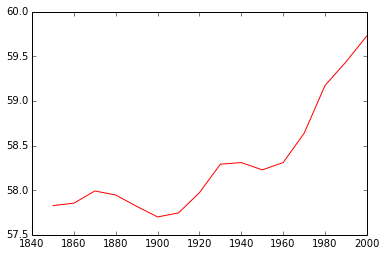
\includegraphics[max size={\textwidth}{\textheight}]{ayocom_sciprog_hw2_tempstd_files/ayocom_sciprog_hw2_tempstd_25_1.png}
    \par
    \end{center}
    
            \end{InvisibleVerbatim}
            
        
    


    % Make sure that atleast 4 lines are below the HR
    \needspace{4\baselineskip}

    
        \vspace{6pt}
        \makebox[0.1\linewidth]{\smaller\hfill\tt\color{nbframe-in-prompt}In\hspace{4pt}{[}262{]}:\hspace{4pt}}\\*
        \vspace{-2.65\baselineskip}
        \begin{ColorVerbatim}
            \vspace{-0.7\baselineskip}
            \begin{Verbatim}[commandchars=\\\{\}]
\PY{n}{plt}\PY{o}{.}\PY{n}{plot}\PY{p}{(}\PY{n}{plotdata}\PY{p}{[}\PY{l+m+mi}{0}\PY{p}{]}\PY{p}{,}\PY{n}{plotdata}\PY{p}{[}\PY{l+m+mi}{2}\PY{p}{]}\PY{p}{,}\PY{l+s}{\PYZsq{}}\PY{l+s}{b}\PY{l+s}{\PYZsq{}}\PY{p}{)}
\end{Verbatim}

            
                \vspace{-0.2\baselineskip}
            
        \end{ColorVerbatim}
    

    

        % If the first block is an image, minipage the image.  Else
        % request a certain amount of space for the input text.
        \needspace{4\baselineskip}
        
        

            % Add document contents.
            
                \makebox[0.1\linewidth]{\smaller\hfill\tt\color{nbframe-out-prompt}Out\hspace{4pt}{[}262{]}:\hspace{4pt}}\\*
                \vspace{-2.55\baselineskip}\begin{InvisibleVerbatim}
                \vspace{-0.5\baselineskip}
\begin{alltt}[<matplotlib.lines.Line2D at 0x106c22950>]\end{alltt}

            \end{InvisibleVerbatim}
            
                \begin{InvisibleVerbatim}
                \vspace{-0.5\baselineskip}
    \begin{center}
    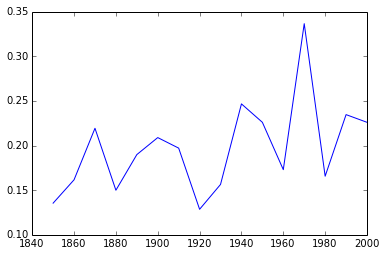
\includegraphics[max size={\textwidth}{\textheight}]{ayocom_sciprog_hw2_tempstd_files/ayocom_sciprog_hw2_tempstd_26_1.png}
    \par
    \end{center}
    
            \end{InvisibleVerbatim}
            
        
    

I still need to figure out how to combine with different vertical
axes.... I am new to python and especially matplotlib.

        

        \renewcommand{\indexname}{Index}
        \printindex

    % End of document
    \end{document}


